\documentclass[conference]{IEEEtran}
\IEEEoverridecommandlockouts
% The preceding line is only needed to identify funding in the first footnote. If that is unneeded, please comment it out.
\usepackage{cite}
\usepackage{amsmath,amssymb,amsfonts}
\usepackage{algorithmic}
\usepackage{graphicx}
\usepackage{textcomp}
\usepackage{xcolor} 
\def\BibTeX{{\rm B\kern-.05em{\sc i\kern-.025em b}\kern-.08em
    T\kern-.1667em\lower.7ex\hbox{E}\kern-.125emX}}
\begin{document}

\title{Overview Of Programming Concepts In Robotics\\}

\author{
    \IEEEauthorblockN{
        Belana Roman
    }

    \IEEEauthorblockA{
        \textit{Institute of Flight Guidance} \\
        \textit{German Aerospace Center DLR}\\
        Brunswick, Germany \\
        Belana.Roman@dlr.de
    }
    \and
    \IEEEauthorblockN{
        Noah Wiederhold
        }
    \IEEEauthorblockA{  
        \textit{In­sti­tute of Flight Sys­tems} \\
        \textit{German Aerospace Center DLR}\\
        Brunswick, Germany \\
        Noah.Wiederhold@dlr.de
    }
}

\maketitle

\begin{abstract}
    This paper gives an overview of the programming concepts in robotics. It is intended to be used as a general source of information. The paper is structured in a way that the reader get to know a number of concepts one at a time. The paper is concluded with a summary of the programming concepts in robotics.
\end{abstract}

\begin{IEEEkeywords}
    robotics, programming, concepts, ai, augmented reality, virtual reality 
\end{IEEEkeywords}

\section{Introduction}
  
\section{Overview of Concepts}

Widely established concepts:

 \begin{itemize}
    \item Online Concepts
        \begin{itemize}
            \item Teach-in
            \item Master-Slave
            \item Vision-Based
        \end{itemize}
    \item Offline Concepts
        \begin{itemize}
            \item CAD/graphical based
            \item text based
            \item task based
        \end{itemize}
    \item Hybrid Concepts
 \end{itemize}

Modern and theoretical concepts:

\begin{itemize}
    \item Semantic Robot Programming
    \item AR
    \item VR
\end{itemize}

\section{Online Concepts}

Programming with online concepts mean working with the active robot and its controls. \cite[p. 186]{b4} %(Grundlagen der Robotik Seite 186)
This concept is used to give a robot a new set of skills in a fast and easy way, where the programmer has the chance to observe the resulting behavior directly.
Commonly used examples of online concepts are Teach-in-Programming and Master-Slave-Programming. \cite[p. 187]{b4}%(" Seite 187)

%general information about online concepts

    \subsection{Teach-in}
        With Teach-in-Programming the programmer teaches the robot needed sequences of movements. Therefore the programmer moves the robot via control elements or buttons, so the system can save the needed movements parameters like position, joint coordinates or the state of grippers and "learn". The movement of the robot can be controlled via consoles or so called "Teach Pendants", handheld programming devices. %(TODO mehr Infos zu Pendant)
        Usually, due to security, the movements are teached with decreased speed. Later on the program paramters like speed or accuracy can be adjusted to meet the needed specifications. Then the programm can be execute automatically, in which the robot moves through all stored positions one after the other and thus executes the planned sequence of movements. \cite[pp. 187-188]{b4} %(" Seite 187-188)
        Usually there are three forms of movements are distinguished:
        \begin{itemize}
            \item Point-to-Point
            \item Continous Path
            \item Muli-Point
        \end{itemize}

        Play-back programming is for example a special from of Teach-in-Programming commonly used for Multi-Point. In this the robot is programmed by demonstrating the movement by touch or hand guidance with switched off actuators. Then the robot stores the positions of the joints and interpolates a smooth path with the given points, which can then be traversed as it was shown. \cite[pp. 188-189]{b4}%(" Seite 188-189)

    \subsection{Master-Slave}
        The Master-Slave-Concept gives the chance to program heavy robots via online programming wihtout having to move them manually. To do this, the programmer needs two coupled robots, a small one that is easy to move and the heavy robot whose capabilities are to be programmed. The programmer moves the small robot, the so called Master. These movements are then copied from the so called Slave, the heavy robot. Because of the need of two coupled robots, this programming concept is usually expensive and therefore only used for teleoperations, so for places humans can not visit easily like under water, irradiated areas or in space. Since the Slave robot is usually very far away, the current scenario of the Slave is usually transmitted to the operator of the Master by camera. Due to transmission delays, the Slave's environment may change faster than the programmer can track it via the camera. This makes accurate movement corrections very difficult. In such cases, special algorithms are used that estimate the future positions of the Slave to make a nearly synchronous control possible. \cite[p. 91]{b6}%(Robotik: Programmierung intelligenter Roboter Seite 91)

    \subsection{Vision-Based}
        Another interesting concept that is not so widely used is vision-based programming. Here, the robot is presented with the action it should perform, which is then detected by various sensors and repeated by the robot until the action meets the expected criteria. \cite[p. 178]{b5} %(Handbuch Robotik Seite 178)
        In the process, the robot must recognise and interpret the relevant features of the movement and objects it needs to interact with in the process, \cite[p. 7]{p4} %(A survey of robot programming systems)
        which makes such a system very complex and computationally intensive. \cite[p. 300]{p5} %(Industrial robot programming by demonstration)

    \subsection{Advantages of online programming}
        A key advantage of online concepts is that no special knowledge in programming is required in order to program the necessary motion sequences into the robot. In addition, the robot is programmed directly in its targeted working environment, so all conditions and possible inaccuracies and disturbance variables can be taken into account directly. \cite[p. 92]{b6} %(Robotik: Programmierung intelligenter Roboter Seite 92)

    \subsection{Disadvantages of online programming}
        Even though online programming makes it possible to specify motion sequences very precisely, this type of robot programming is not useful or even possible for all applications. This concept makes it impossible, for example, to control the program flow beyond the movements, to process sensor data or to perform mathematical calculations. In addition, online programming requires time, which is a great disadvantage within a manufacturing process. Within this time, the robot is withdrawn from the process or possibly the whole process has to be stopped for this time. For such problems, concepts of offline programming are used. \cite[pp. 190-191]{b4}%(Grundlagen der Robotik Seite 190-191)

\section{Offline Concepts}

    Programming with offline concepts means programming the robot without the need to be in direct contact with an active robot. This concept is used to give a robot a new set of skills in an indirect way, without interrupting the overall production process.
    The finished program gets loaded onto the robot afterwards, resulting in a minimum of downtime of other processes. \cite[p. 186]{b4}

    \subsection{text based}

        The concept of text based programming is based on the idea of programming a robot by manually writing source code in the native language of the robot or a language which can be translated into the native ones. The source code containing a set of instructions gets compiled like in any other programming language and the resulting program gets loaded onto the robot. %cite this?
        This explicit programming approach is one of the oldest and most common programming concepts in robotics. %cite this?

        % what are problem solving languages?
        Most of the programming languages used in robotics are problem-solving languages, which means, that they contain special commands for certain tasks the robot can perform. A basic example would be a command for moving the robot from one point to another. This is commonly done by giving the coordinates of the initial point, a target point and arguments for how to interpolate between those points as parameter to the command. 
        The robot then calculates the path based on the parameters and moves accordingly. %cite this?
               
        Based on the 2019 market share of today's biggest robot manufacturers the most common languages used for text based programming are RAPID, KRL and KAREL. \cite{s1}

        For those languages many programming environments exist. Examples based on the mentioned would be RobotStudio from ABB, Officelite from KUKA and ROBOGUIDE from FANUC.

        In addition to the textual programming features most of the enviroments also offer a graphical programming interface.
        The main concepts used in these interfaces are controlling the robot by draggable points or with a simulated controller.
        The first method works by moving and rotating of for example the robot's arm on different axis. 
        The second approach is based on simulated controller similar to the ones used in teach-in programming of the robot.

        Some environments even make use of AR technologies to show and simulate the robot running the created program in the real world.
        
        %example robot studio %cite this

    \subsection{task based}

        Task based programming is a more abstract and implicit approach to programming a robot.
        Instead of describing what movement the robot should perform it defines the tasks the robot should perform.
       
        In comparison to text based programming it adds a layer of abstraction to the programming workflow. For example wouldn't you have to understand the complex physic when gripping an object any more, you could just use some kind of grip command which does the task for you. %cite

        Task based programming typically uses sensor information to add dynamic to the program while running. For example if the robot is supposed to pick up an object whose position is not precisely known, it would first check if the object is in the gripper and if not it would move to the object and pick it up. If the object is already in the gripper it would just move to the next task.
        %cite

        Again there are many different programming environments for task based programming. Some examples are RoboGuide from FANUC and Visual Components. RoboGuide defines tasks by using a drag and drop interface, these task can later be combined to form a program.
        Visual Components instead defines tasks by a flowchart.
        %cite

        The resulting task descriptions get translated into lines of code by a task transformer. These code lines then get processed like in the text based programming approach by compiling it. %cite this?

        

    \subsection{CAD/graphical based}

        CAD based programming environments offer a mathematical approach to the programming workflow by adding different models and CAT based tools.
        Models could range from simple models of movements to more complex simulation models of the environment and the robot itself. %TODO cite this

        %add to this?

        In addition to the pure simulation of mathematical models, graphical based programming environments add a time component to the simulation, making their simulation a 4D scene.
        They contain a kind of 3D scene viewer and offer the features to simulate not only one robot and its movements but also the whole production environment. This allows the user to simulate the whole production process and interactions between different parts of the production environment. %cite

        An example for a graphical programming environment is Visual Components. %cite

\section{Hybrid Concepts}

    Hybrid concepts combine the advantages of both offline and online concepts.
    This could for example be done by creating a general program offline and later  fine tune this program with online concepts on the real robot or the other way around by first programming the robot online and then optimizing the program offline.
    \cite[p. 186]{b4}

\section{Modern Concepts} %?

    \subsection{Semantic Robot Programming}

        The concept of semantic programming is a new approach to programming robots based on demonstrating.

        Recently the authors of \cite{p1} proposed a new concept of programming robots by demonstrating the desired behaviour to the robot by giving an initial state and a goal state for which the robot has to find the best way to get from the initial state to the goal state

        They used a new scene estimation method called DIGEST which splits the scene into a scene graph representing the structure of the initial state. The only parameter needed is the information about the number of objects present in the scene. The scene graph is then used to find the best way to get from the initial state to the goal state.
        For that a task planner is used which generates a series of actions to accomplish the task. These actions are then executed by the robot. %cite this?
        \cite[p. 2]{p1}

    \subsection{AR}
    
        The concept of programming robots by using AR is another new approach to programming robots.
        The general idea of AR is to integrate additional information into the real world. In our specific case this could be an overlay of the robot adding methods to control the robot.
        The authors of \cite{p3} proposed a concept of how this could be done using a HoloLense from Microsoft.
        For example did they add the ability to specify a pickup and a place location. This allows for an automatic path generation. The path then gets visualized in the HoloLense display. The user can edit this path by gestures and the movement of the robot can be simulated.
        If the user is satisfied with the path the robot can be instructed to execute the path with a voice command. %cite this?
        \cite[p. 2]{p3}

        They found that the time needed to teach a robot using their AR based method was significantly shorter than with the traditional kinesthetic teaching approach. 
        They also found that the average completion rate was significantly higher in a task containing movements where the path has to be made out of a high amount of distinct points, for example a sin. Using the AR method led to users placing more points on the path as it was easier to do so, resulting in better results in the sin movement.
        \cite[pp. 4-5]{p3}

    \subsection{VR}

        (p2)


\section{Conclusion}

    Generally programming robots is still a complex task and can be done in many ways. 
    In the past the programming of robots was done by experts who had to know the complex physics of the robot and the environment. Modern concepts nowadays tend to simplify this task by adding abstraction layers or high level methods like AR or VR to the programming workflow. This allows for a more intuitive programming workflow and makes it easier for non experts to program robots. Modern concepts also help to reduce costs and time needed to program a robot, making the usage of robotic more accessible for small- and medium-sized companies.
    Nevertheless, there are still many challenges to overcome before programming robots becomes a simple task for everyone. For example the usage of AR and VR is still limited to a few experimental environments and the usage of semantic programming is still in its infancy. Would these concepts improve in functionality and usability and become more widespread, they could be a big step towards a more accessible programming of robots.

\nocite{*}

\bibliographystyle{unsrt}
\bibliography{quellen}


\cleardoublepage
\appendix

\section{Appendix}
    % \begin{figure}[htbp!]
    %     \centering
    %     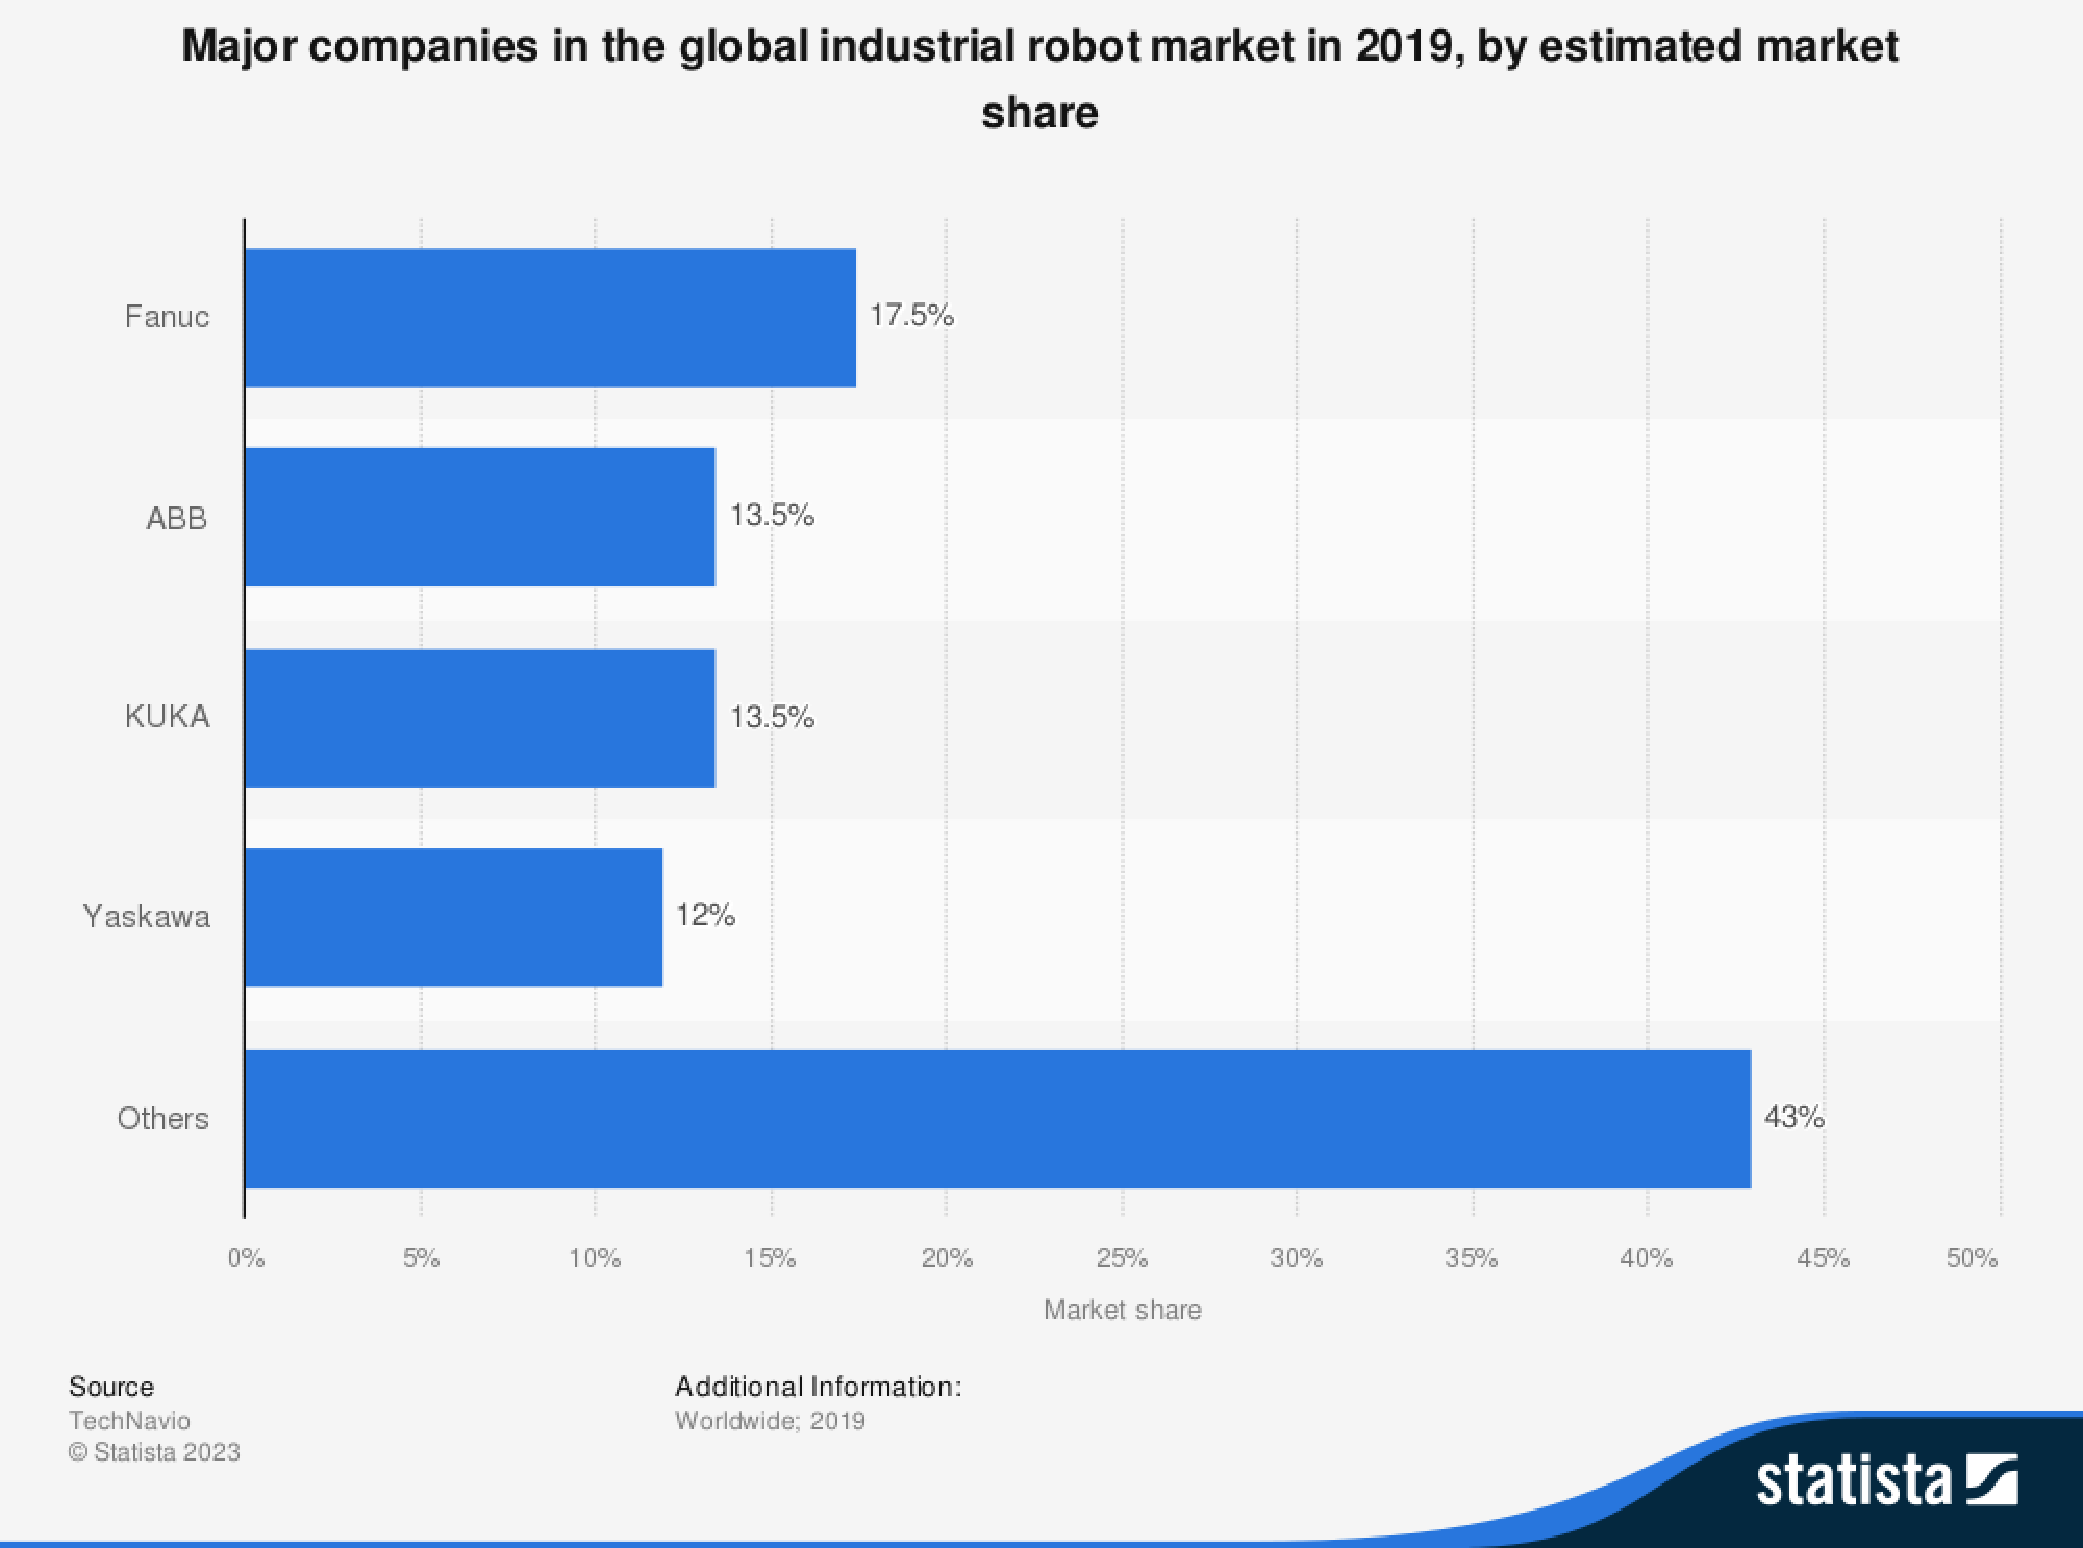
\includegraphics[scale=0.25]{./Moderne_Konzepte_Quellen/Citavi Attachments/statistic_id317178_global-industrial-robot-market-major-companies-by-market-share-2019.pdf}
    %     \caption{Stastic about the market share of the biggest robot manufacturers in 2019 \cite{s1}}
    %     \label{fig}
    % \end{figure}

\end{document}


